
\section{Introduction} \label{sec:Introduction}

It is generally agreed upon that large-scale, universal quantum computing will require comprehensive error correction \cite{Wang2011,Fowler2012}.





There has been a recent proposal to make use of dopants in silicon to act as qubits \cite{the paper} to implement a version of the surface code. 


We have simulated a probe qubit interacting with four data qubits. The probe qubit is performing a circular orbit $40$ nm above the data qubits, and in this document we will document the effect of various errors. These errors include dephasing, dopan placement uncertainties and a path jitter. 



\subsection{The surface code}


\subsection{A physical implementation}\label{sec:PhysicalImplementation}
In a paper in 2015, it awas proposed by G'Orman \textit{et al}. 

Let us first take a closer look at the scheme proposed in \cite{the paper}. The data qubits are dopants placed in silicon placed in a square pattern using the best dopant placement techniques available, which currently stand at [insert some error value and cite it]. To perform the stabiliser measurements, a probe qubit of a different dopant species is placed on a mobile slab above the data qubits. Each probe qubit performs a stabiliser measurement on four data qubits, a procedure which is performed by physically moving the overhead slab with the probe qubits. 

Some differences in physical parameters are required. 


\begin{figure}[H]
	\centering
	\subfloat[]{ 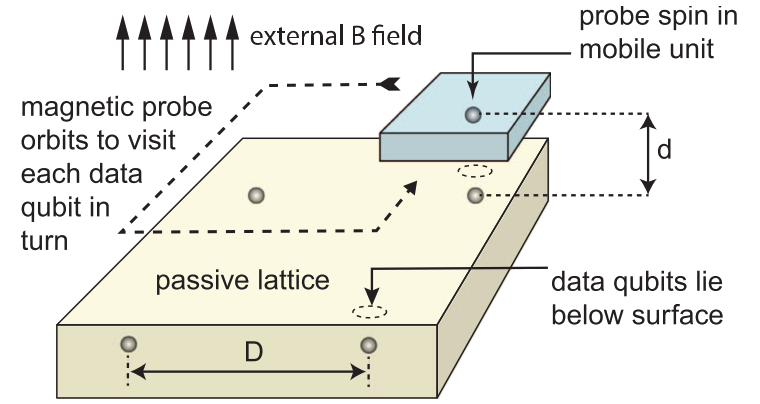
\includegraphics[width=0.8\linewidth]{../Figures/paper-parity} \label{FIG:paper-parity}}\\
	\subfloat[]{ 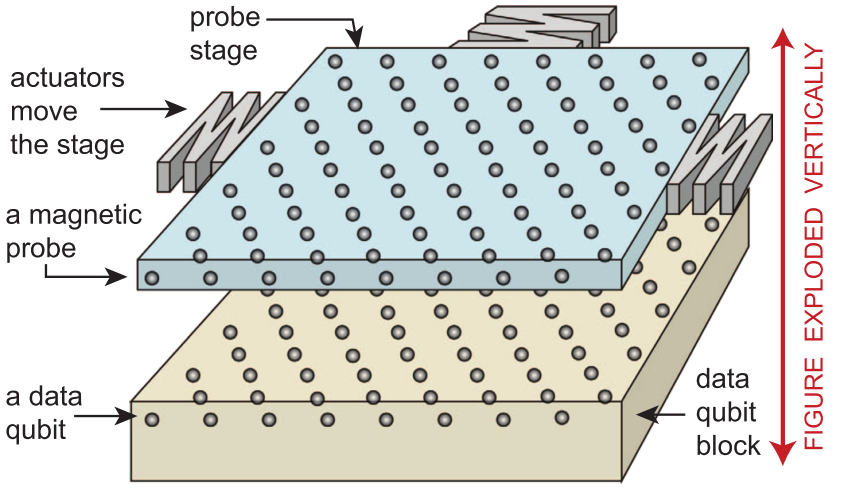
\includegraphics[width=0.8\linewidth]{../Figures/paper-mems} \label{FIG:paper-mems}}
	\caption[oddeven]{}
	\label{FIG:paper}
\end{figure}
